\documentclass[11pt,a4paper]{article}
\usepackage[utf8x]{inputenc}
\usepackage[T1]{fontenc}
\usepackage{mathptmx}
\usepackage{graphicx}
\usepackage[pdftex,linkcolor=black,pdfborder={0 0 0}]{hyperref} % Format links for pdf
\usepackage{calc} % To reset the counter in the document after title page
\usepackage{enumitem} % Includes lists
\usepackage{caption}
\captionsetup[figure]{font=small,labelfont=small,labelfont=bf}
\usepackage{subcaption}
\usepackage{amsmath}
\usepackage{amssymb}
\usepackage{amsfonts}
\usepackage{fancyvrb,newverbs,xcolor}
\usepackage{verbatim}
\definecolor{cverbbg}{gray}{0.93}

\newenvironment{lcverbatim}
 {\SaveVerbatim{cverb}}
 {\endSaveVerbatim
  \flushleft\fboxrule=0pt\fboxsep=.5em
  \colorbox{cverbbg}{%
    \makebox[\dimexpr\linewidth-2\fboxsep][l]{\BUseVerbatim{cverb}}%
  }
  \endflushleft
}

\renewcommand\thesection{Task \arabic{section}}
\renewcommand\thesubsection{\alph{subsection}.)}
\renewcommand\thesubsubsection{\Roman{subsubsection}:}

\frenchspacing
\linespread{1.2}
\usepackage[a4paper, lmargin=0.12\paperwidth, rmargin=0.12\paperwidth, tmargin=0.05\paperheight, bmargin=0.1\paperheight]{geometry}

\usepackage[all]{nowidow} % Tries to remove widows
\usepackage[protrusion=true,expansion=true]{microtype}

\title{Exercise 4}
\author{Kai Schneider}
\date{\today}

\begin{document} 

\maketitle

\section{}

\subsection{Advantages MC vs DP}

\begin{itemize}
    \item MC only considers values from one episode for it's updates, not from all previous backups\\
    Although this might increase variance, it drastically improves computation time
    \item For DP we need the transition matrix/distribution, which might be unrealistic for real 
    scenarios.\\
    For MC we try to obtain our information by interacting with the environment. 
\end{itemize}

\subsection{Example environment}
MC methods are only suitable for repetitve scenarios, because we only update after an episode has ended.\\
The most common examples are games like blackjack or backgammon where it is close to impossible to 
determine the value of the current state. Therefore DP isn't a viable option, but MC is.\\
A more exotic example environment might be the simulation of illumnation/reflection behaviours. Approximating the
path of the light with MC is an efficient way to solve this problem because we don't have to solve
the infinity number of possible situations (angle, reflectivity, intensity, etc) or create an complex
simulation model of the system.


\section{}

\subsection{first visit MC}

\subsubsection{10k episodes}

\begin{figure}[h!]
  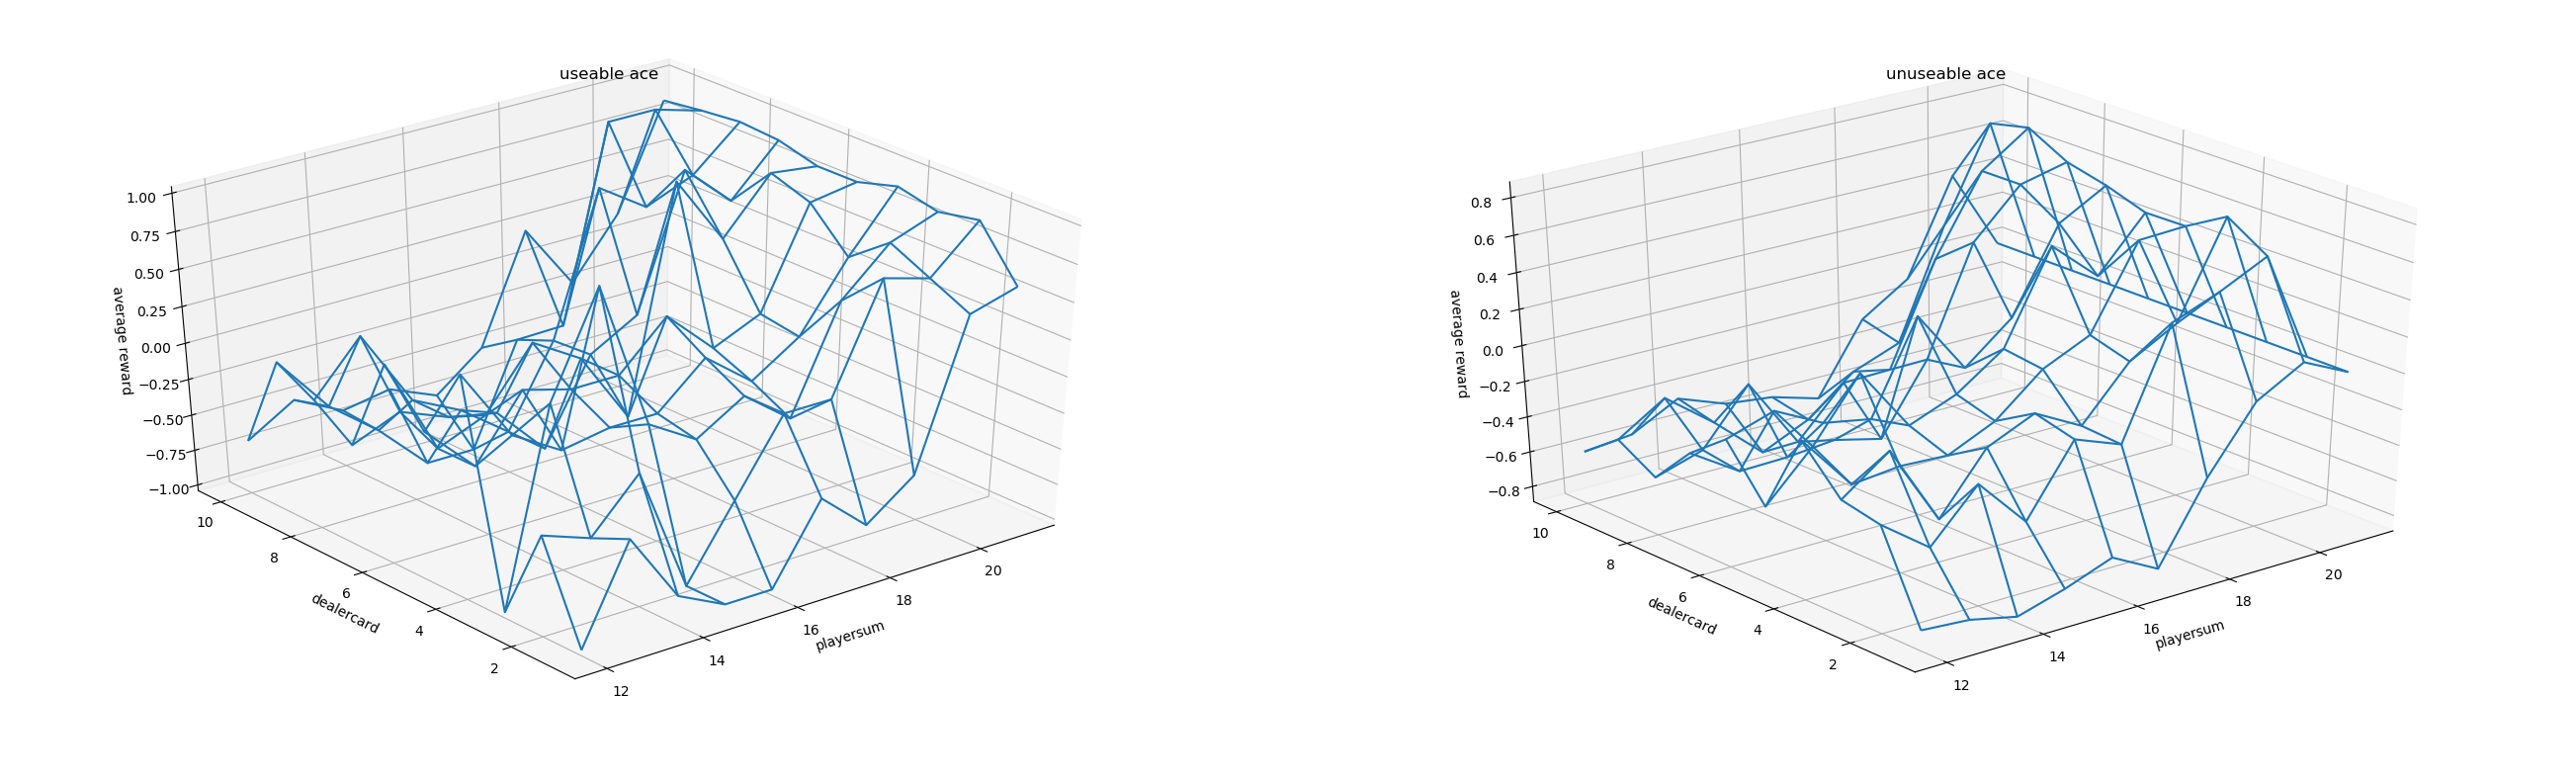
\includegraphics[width=.7\textwidth]{10k_eps.png}
  \centering
  \caption{plots first-visit MC with 10k episodes (usable ace left, unusable right)}
  \label{fig1}
\end{figure}

\subsubsection{500k episodes}

\begin{figure}[h!]
  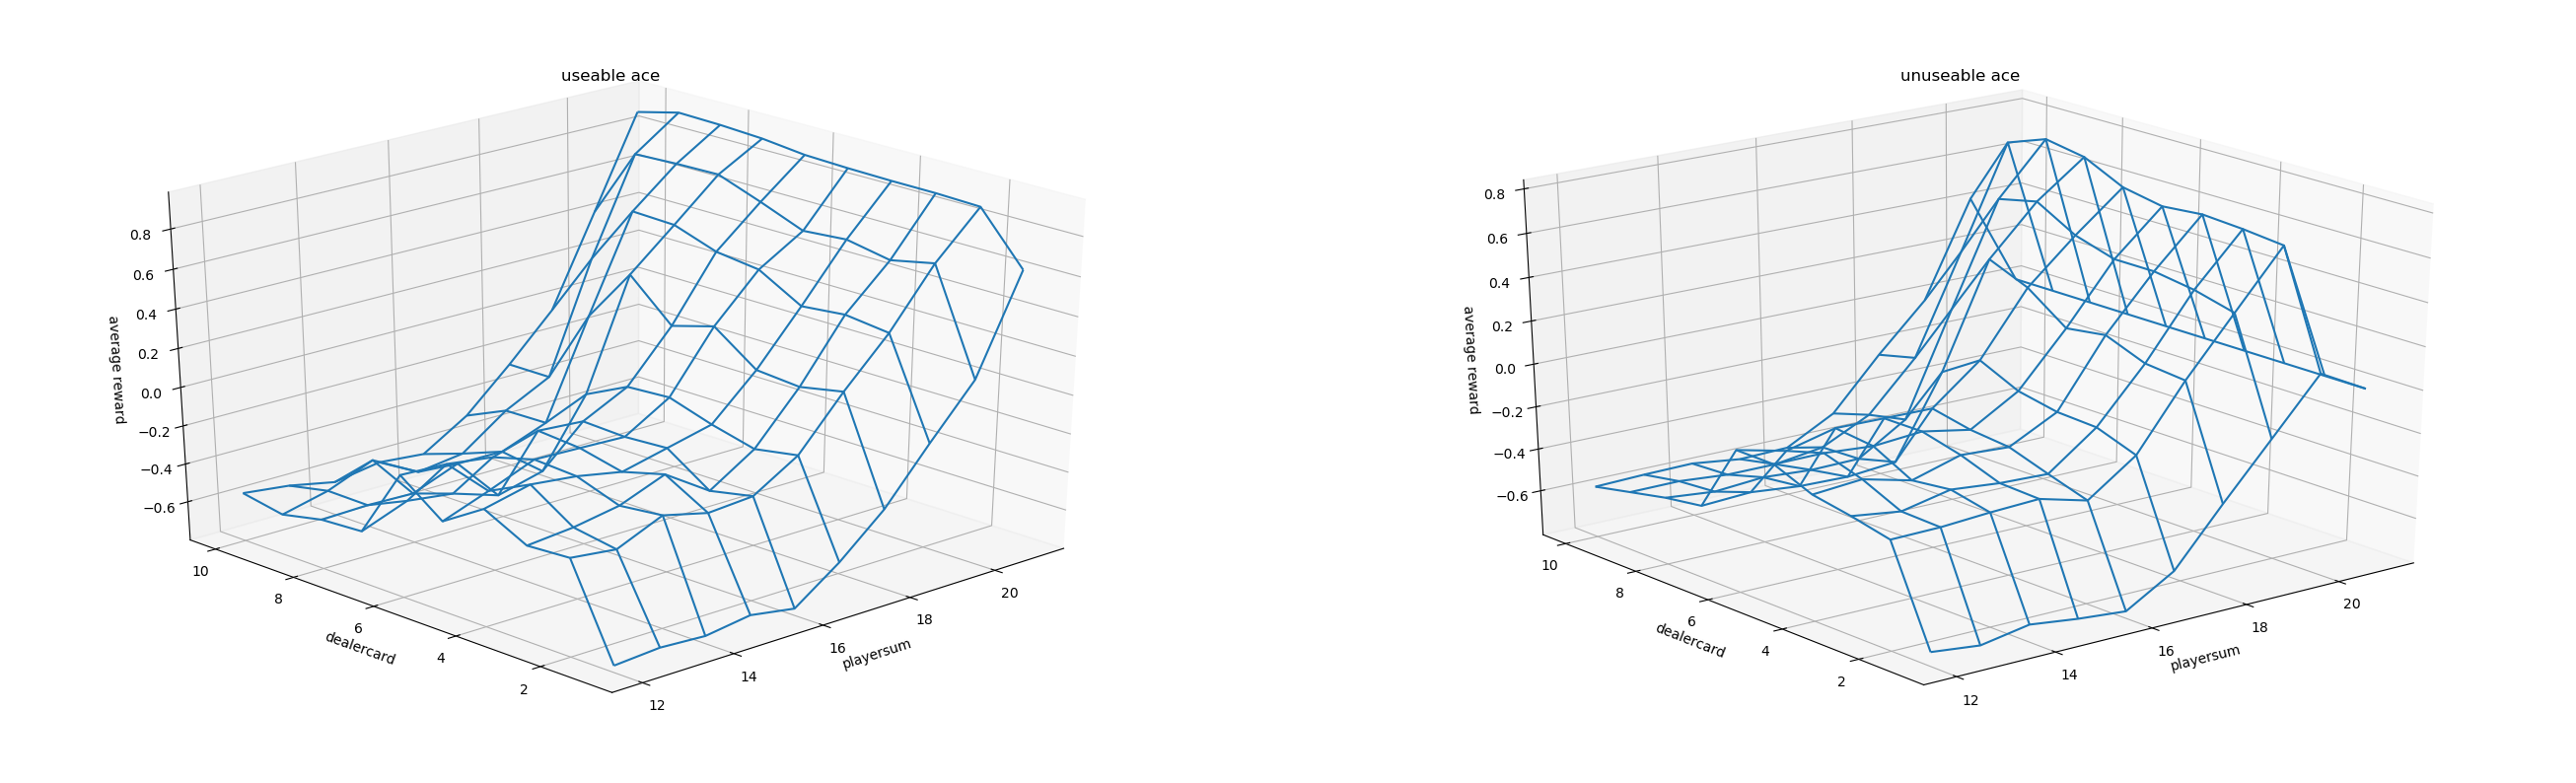
\includegraphics[width=.7\textwidth]{500k_eps.png}
  \centering
  \caption{plots first-visit MC with 500k episodes (usable ace left, unusable right)}
  \label{fig2}
\end{figure}

\subsection{ES MC}

For all plots:
\begin{itemize}
  \item \textbf{Yellow:} 1.0 - hit
  \item \textbf{Purple:} 0.0 - stick
\end{itemize}


\begin{figure}[h!]
  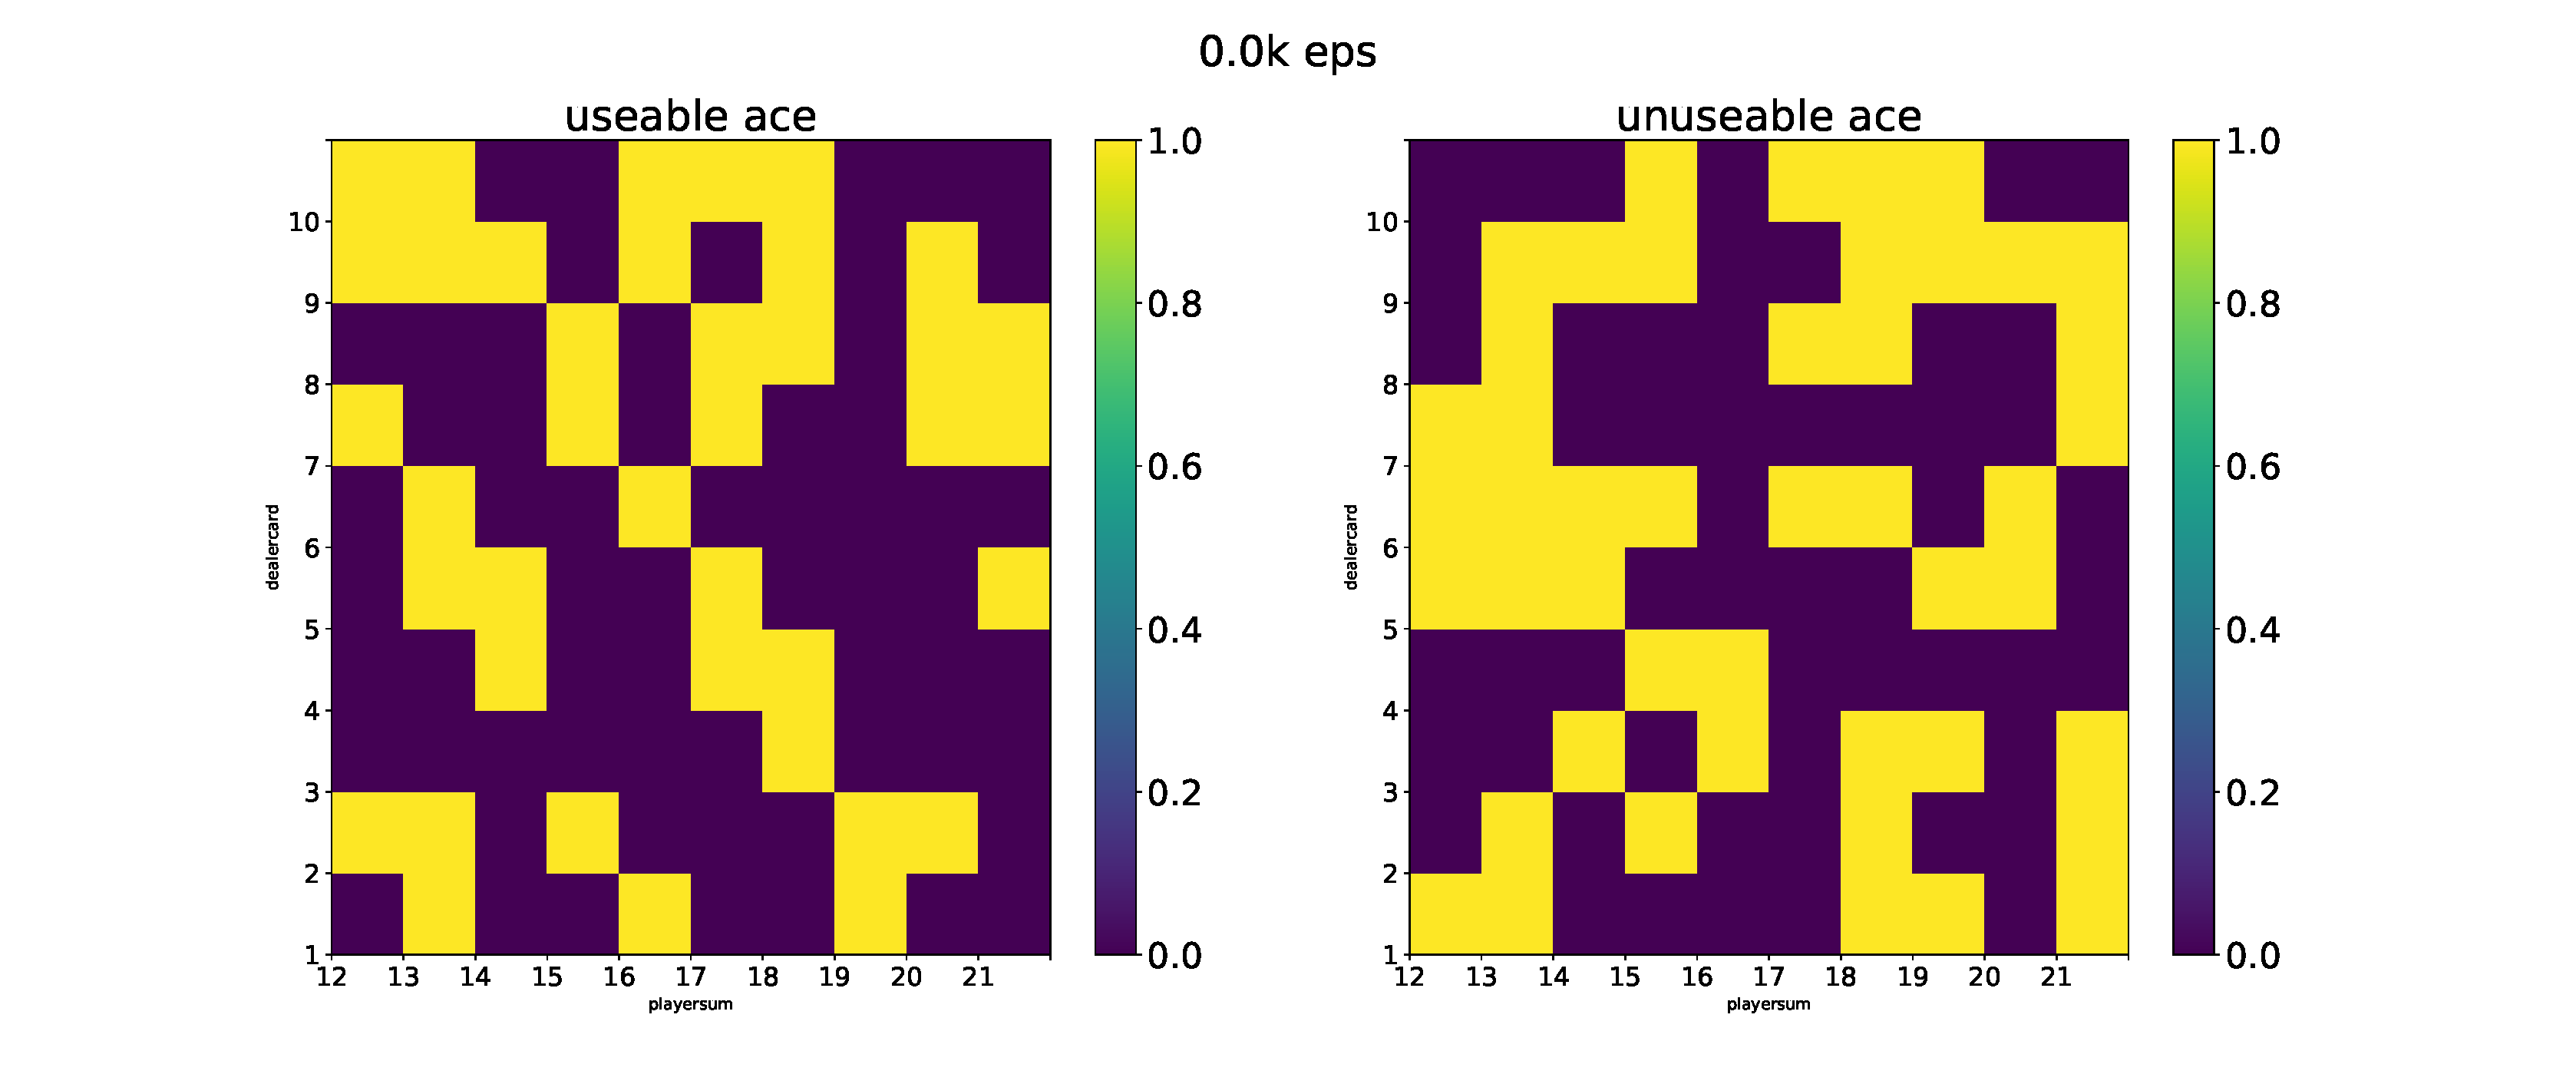
\includegraphics[width=.7\textwidth]{es-v3-0k.eps}
  \centering
  \caption{plots ES MC with 0k episodes (usable ace left, unusable right)}
  \label{fig3}
\end{figure}

\begin{figure}[h!]
  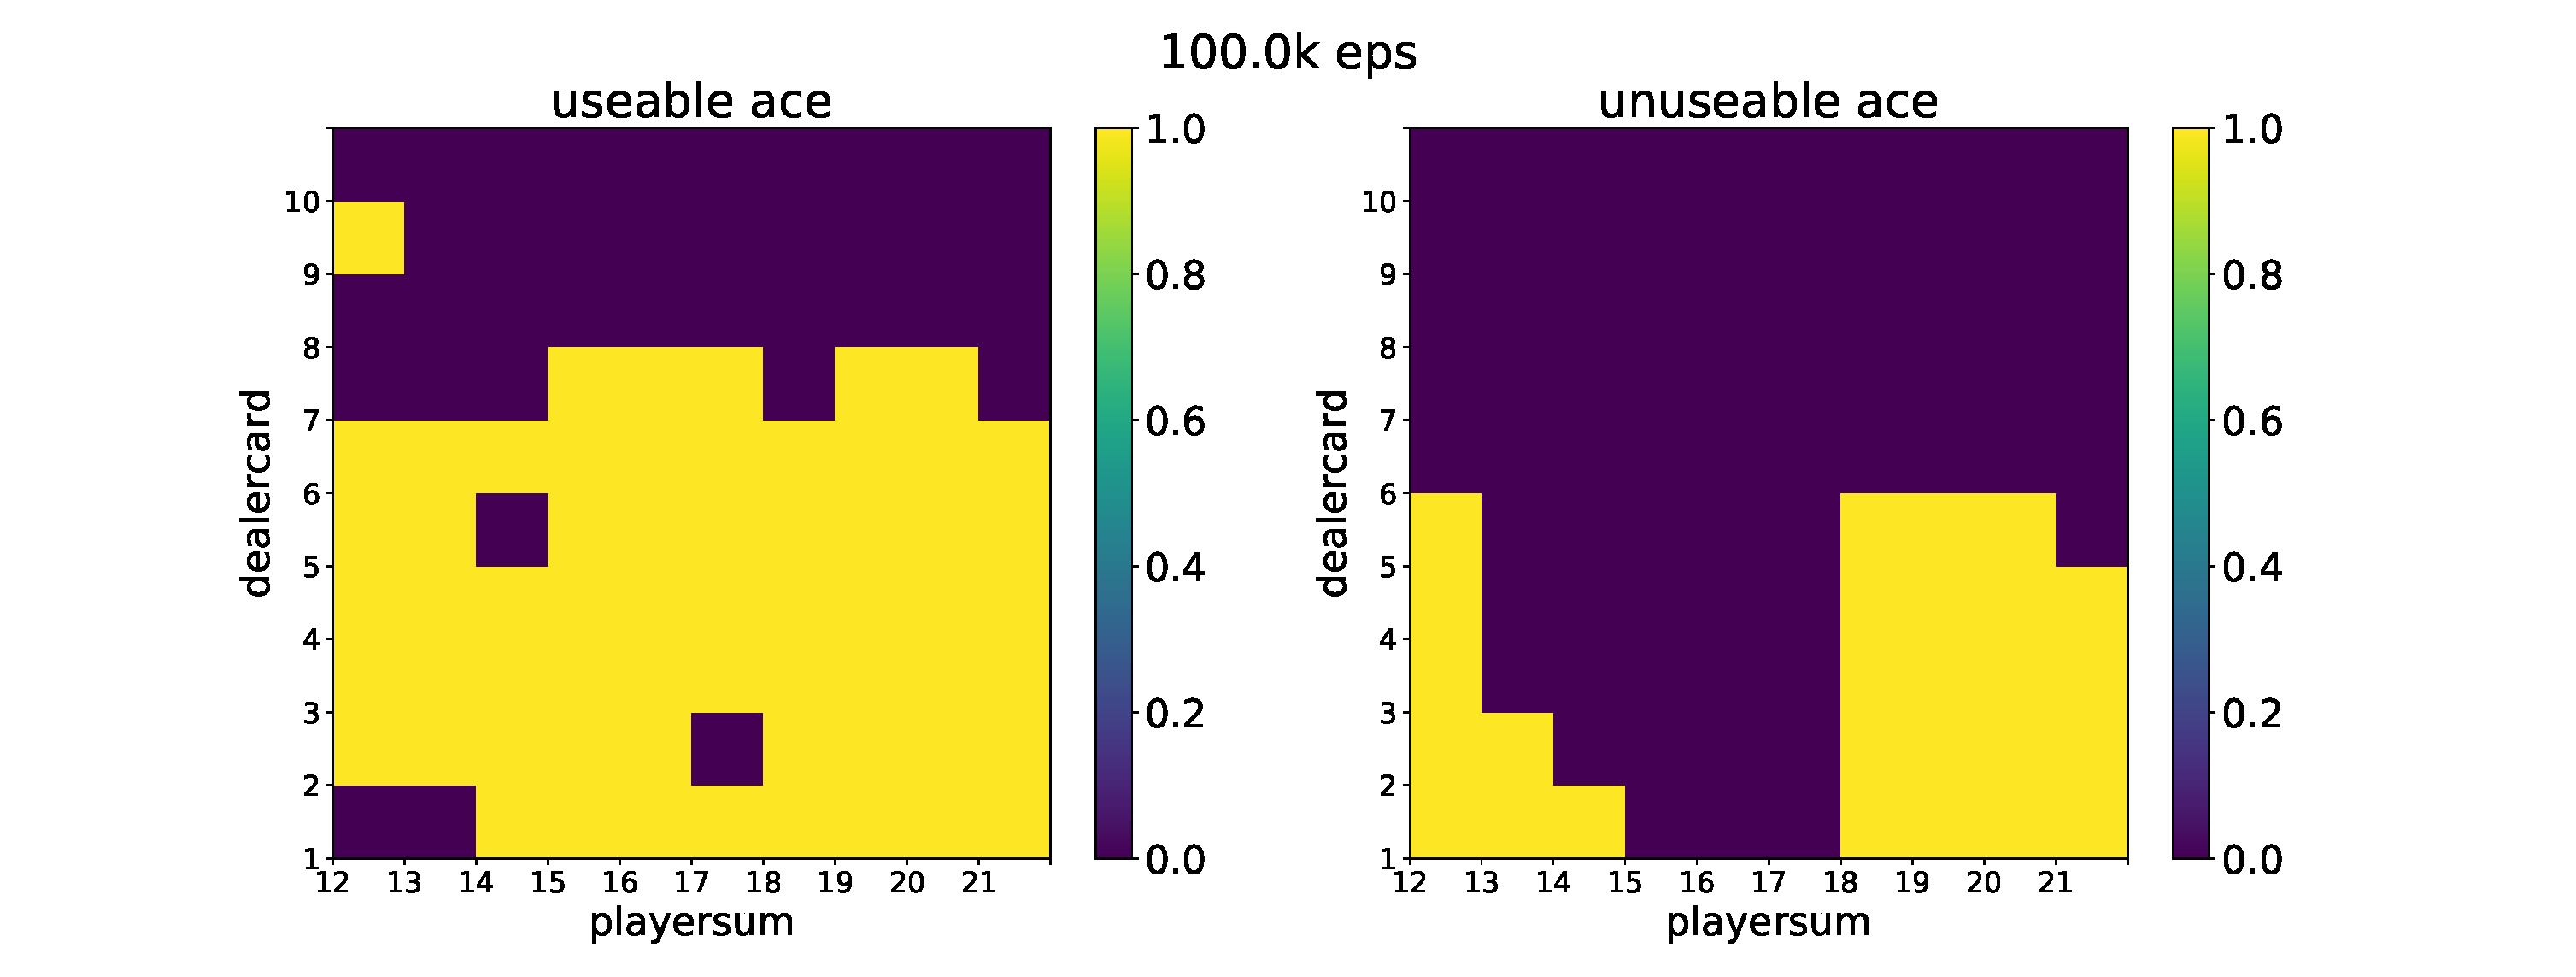
\includegraphics[width=.7\textwidth]{es-v3-100k.eps}
  \centering
  \caption{plots ES MC with 100k episodes (usable ace left, unusable right)}
  \label{fig4}
\end{figure}

\begin{figure}[h!]
  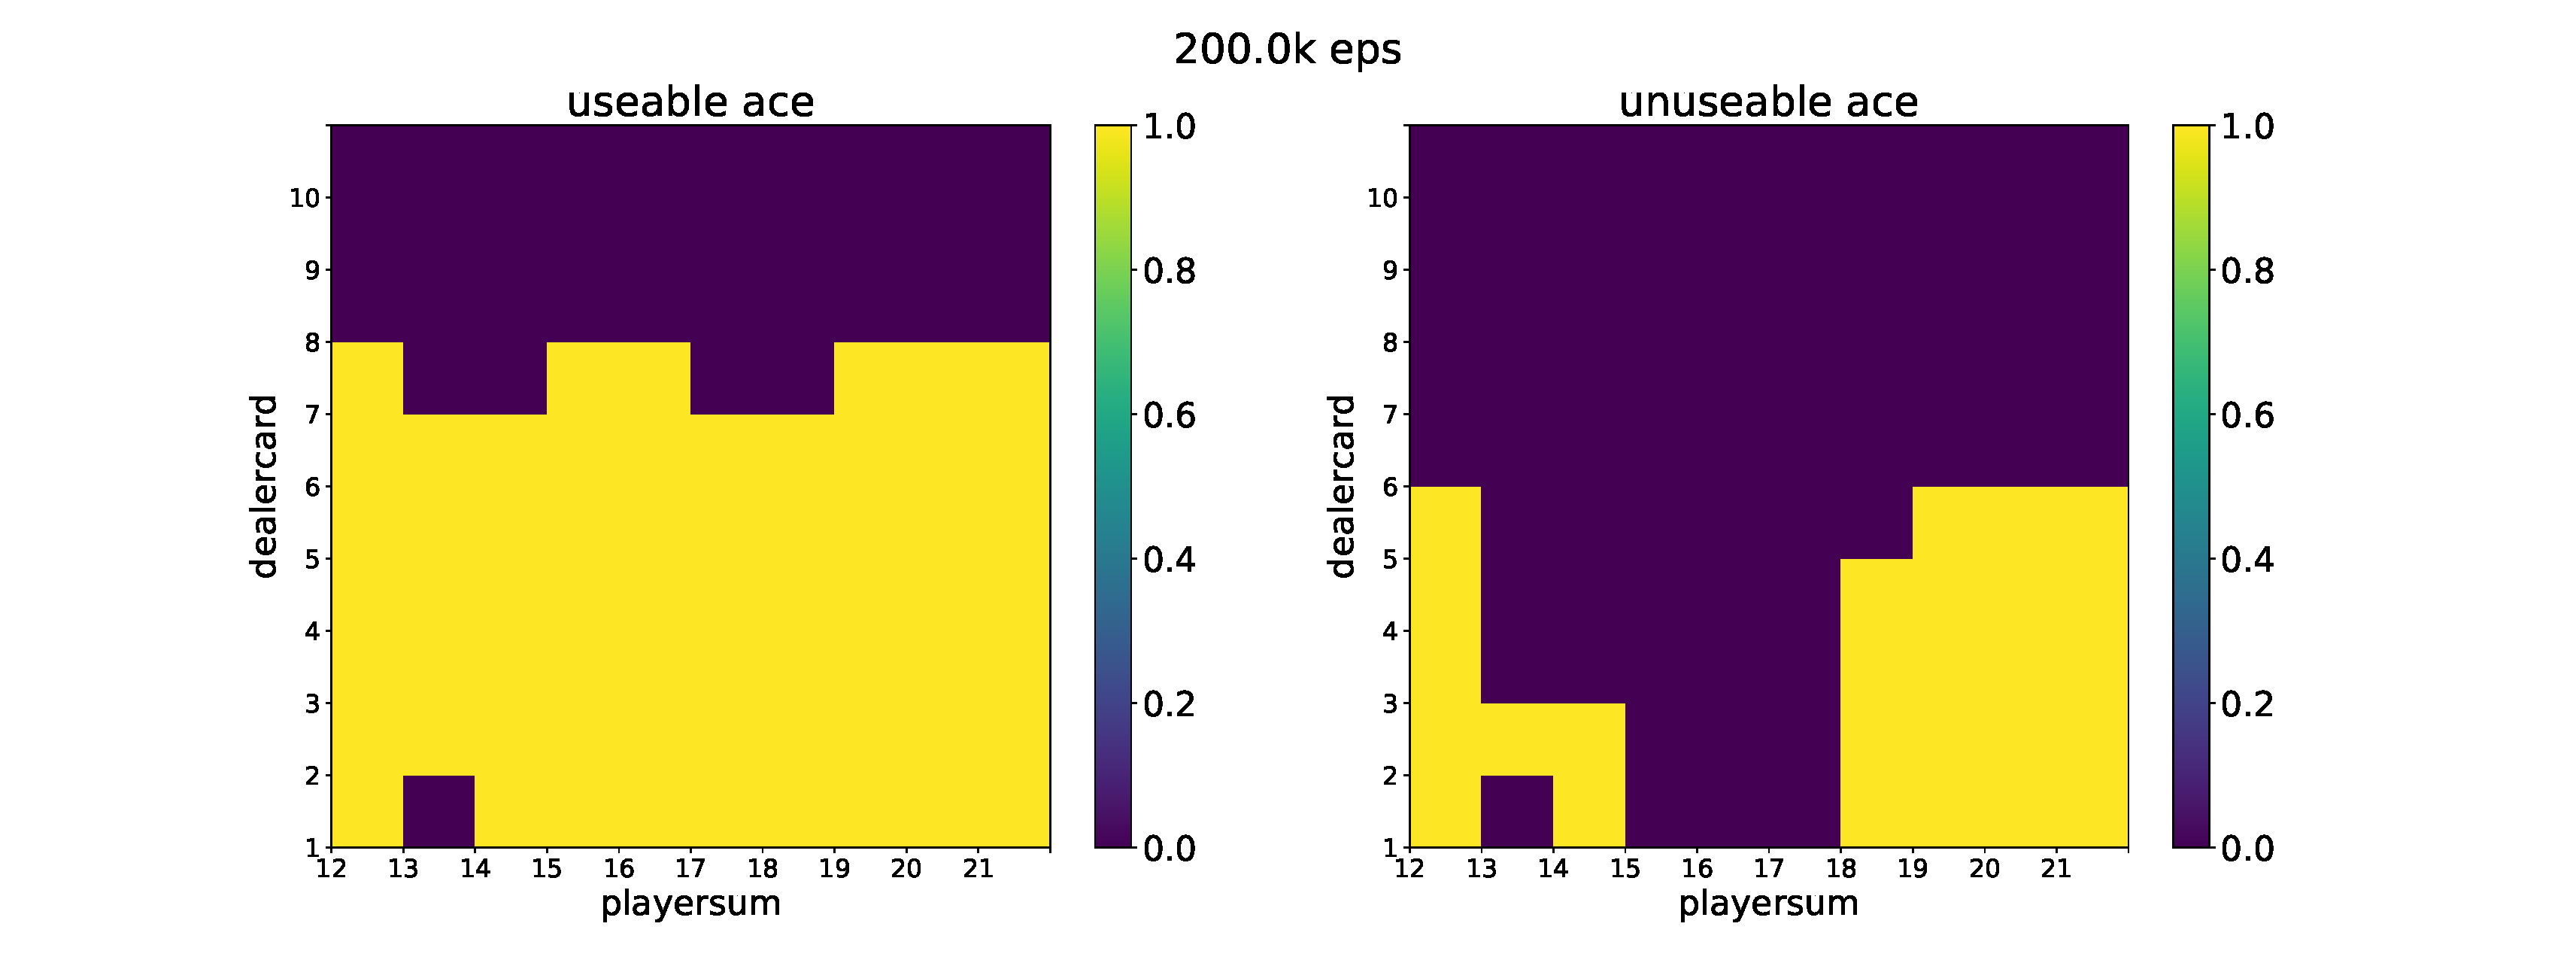
\includegraphics[width=.7\textwidth]{es-v3-200k.eps}
  \centering
  \caption{plots ES MC with 200k episodes (usable ace left, unusable right)}
  \label{fig5}
\end{figure}

\begin{figure}[h!]
  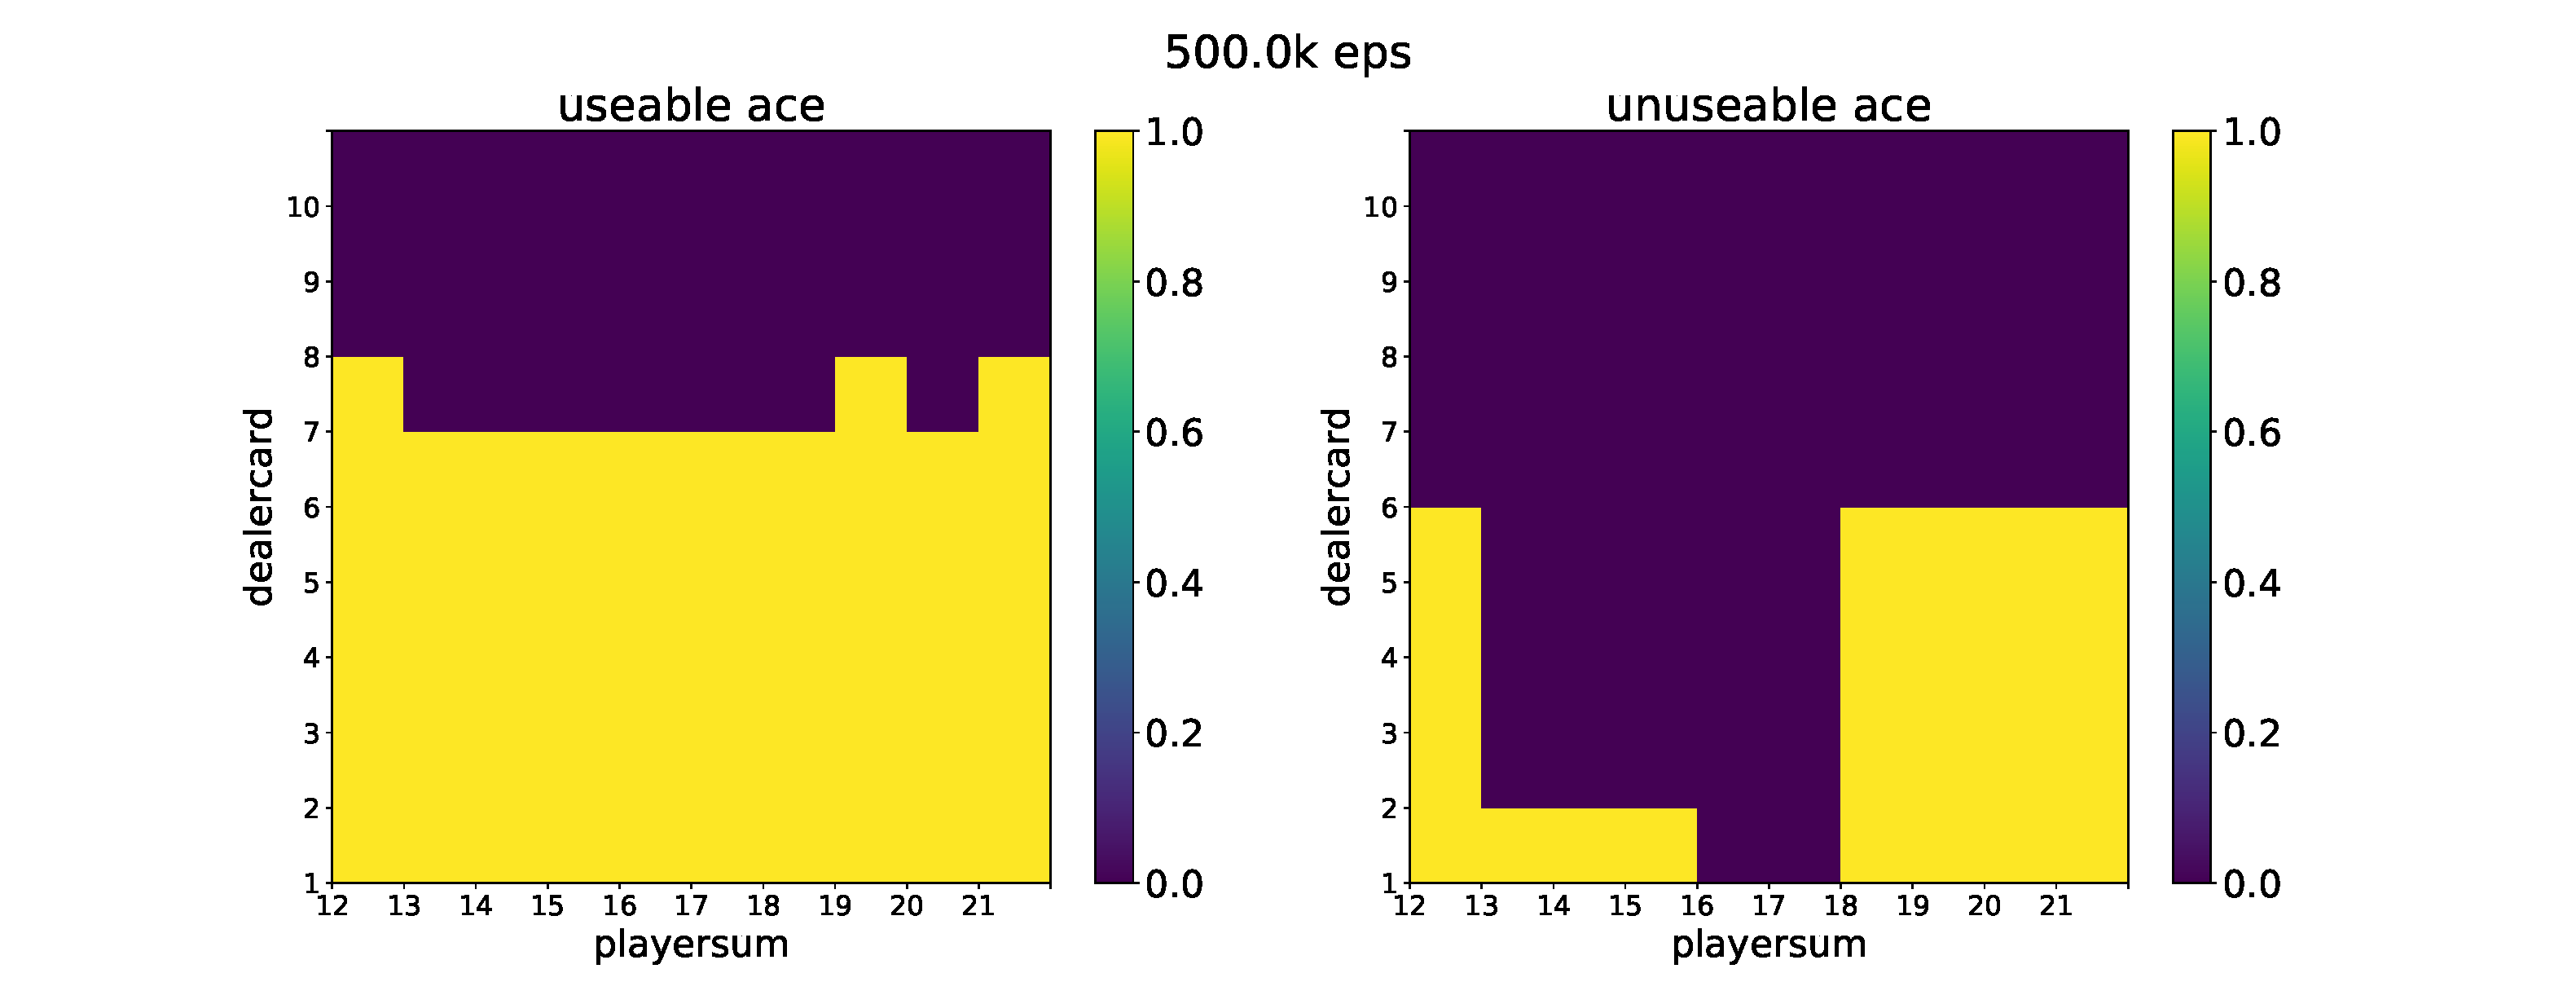
\includegraphics[width=.7\textwidth]{es-v3-500k.eps}
  \centering
  \caption{plots ES MC with 300k episodes (usable ace left, unusable right)}
  \label{fig6}
\end{figure}

\begin{figure}[h!]
  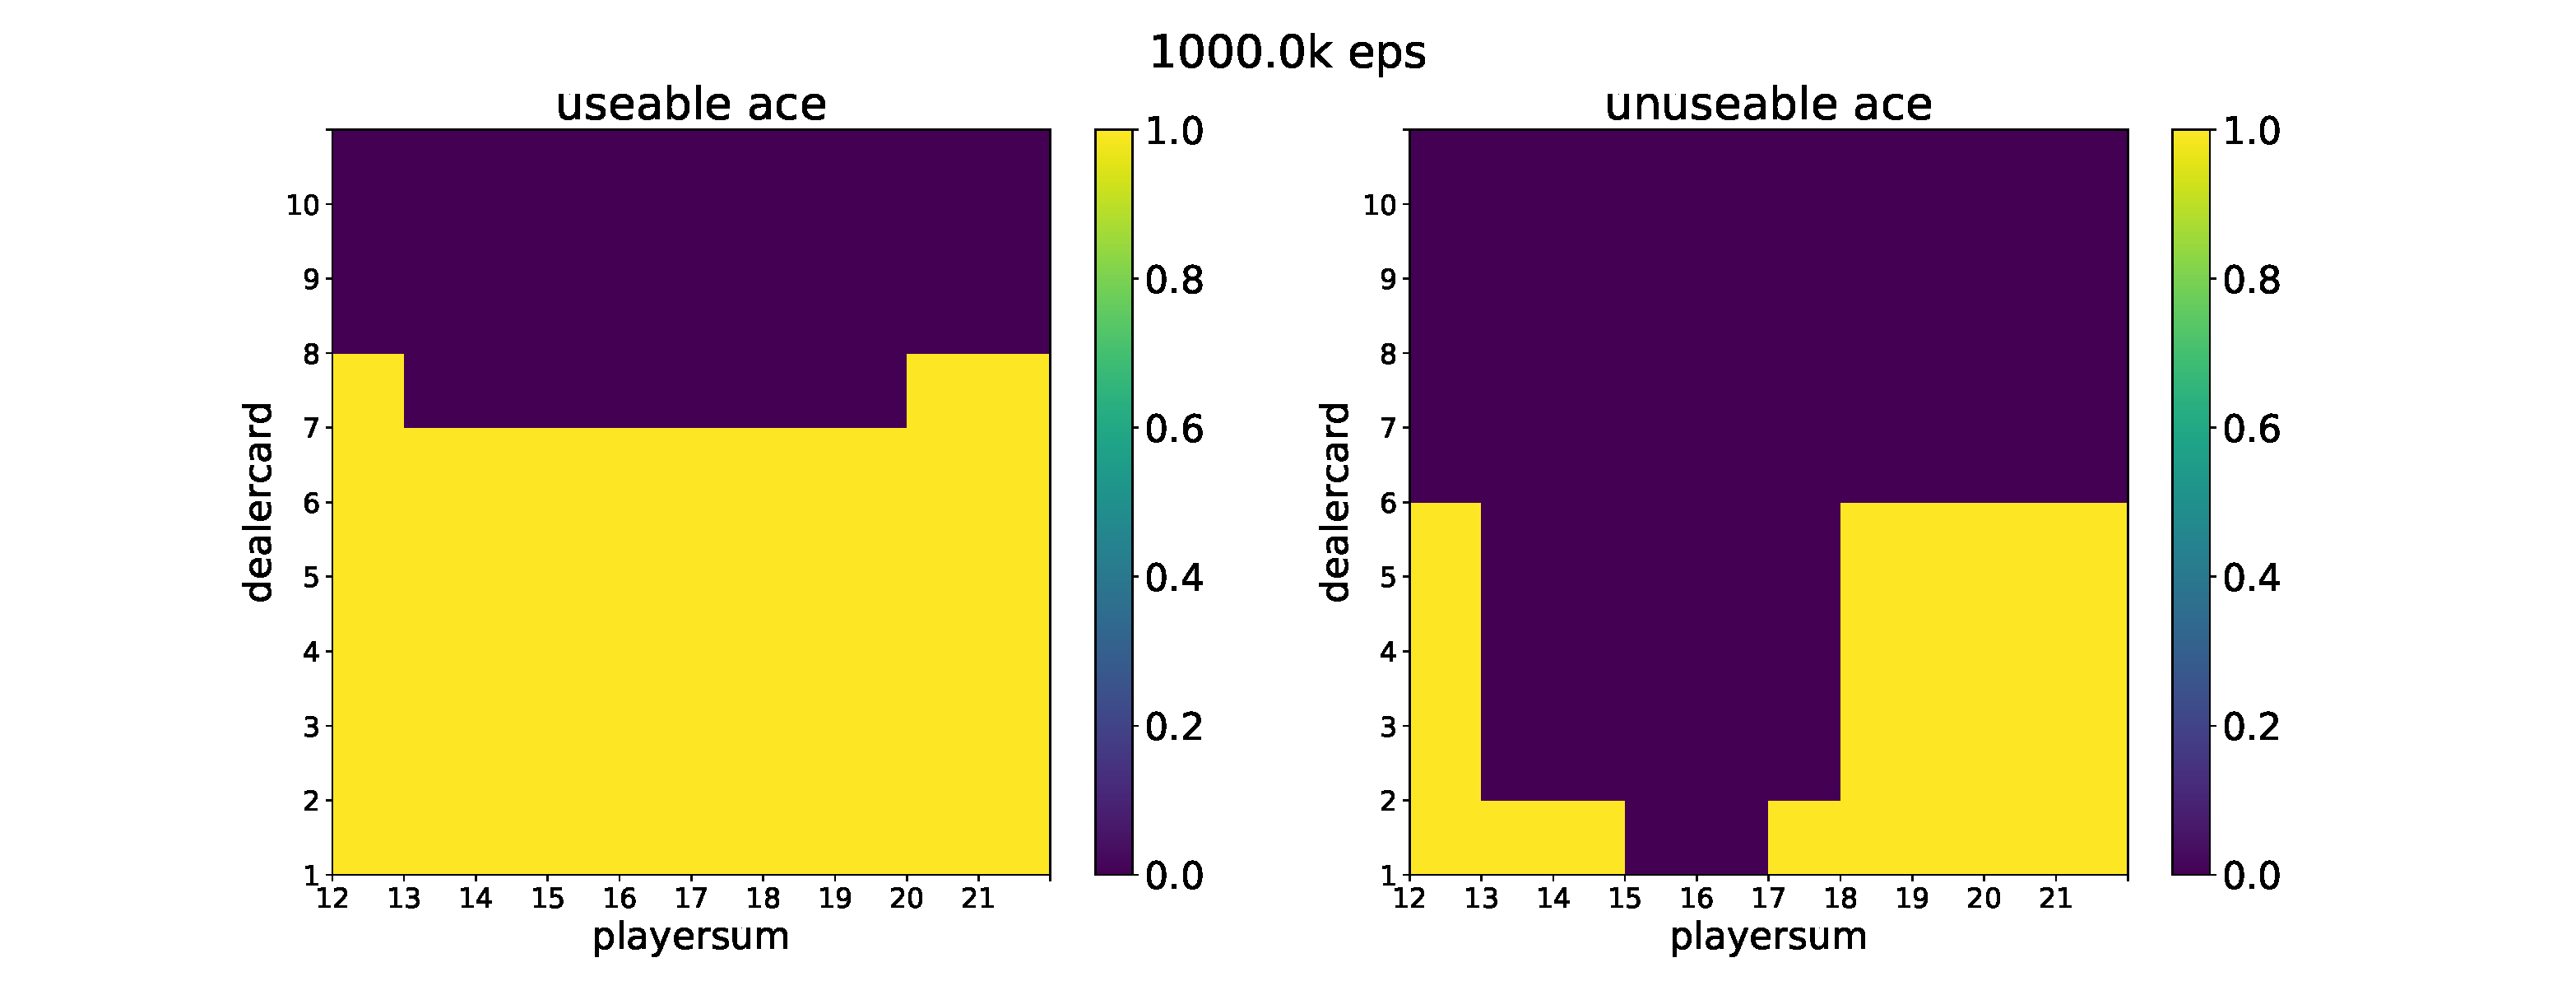
\includegraphics[width=.7\textwidth]{es-v3-1000k.eps}
  \centering
  \caption{plots ES MC with 400k episodes (usable ace left, unusable right)}
  \label{fig7}
\end{figure}


\end{document}

